\documentclass[border=2pt]{standalone}
\usepackage{tikz}
\usetikzlibrary{positioning, fit, shapes, arrows, calc}

\pgfdeclarelayer{bg}    % declare background layer
\pgfsetlayers{bg,main}  % set the order of the layers (main is the standard layer)

\newcommand{\coula}{0785F2}
\newcommand{\coulb}{F29F05}
\newcommand{\coulc}{F21313}
\newcommand{\could}{E6F21F}



\definecolor{part1}{HTML}{\coula}
\definecolor{part2}{HTML}{\coulb}
\definecolor{part3}{HTML}{\coulc}
\definecolor{part4}{HTML}{\could}

\begin{document}
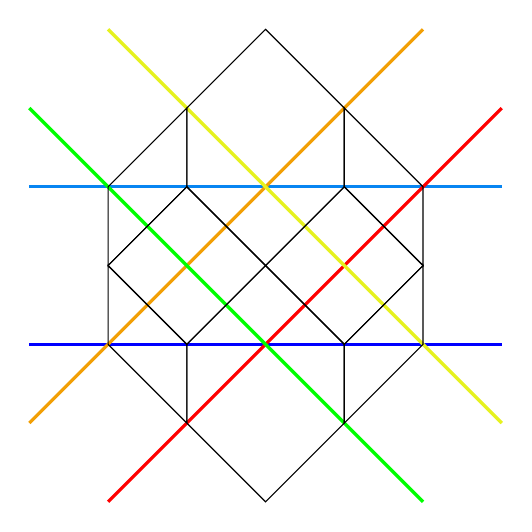
\begin{tikzpicture}
\coordinate (C) at (180:1);
\coordinate (D) at (90:1);
\coordinate (E) at (-90:1);
\coordinate (F) at (0:1);
\coordinate (A) at ($2*(C)+(D)$);
\coordinate (Ag1) at ($(A)+(C)+(D)$);
\coordinate (Ag2) at ($(A)+(C)$);
\coordinate (B) at ($2*(C)+(E)$);
\coordinate (Bg1) at ($(C)+(B)$);
\coordinate (Bg2) at ($(C)+(B)+(E)$);
\coordinate (G) at ($2*(F)+(D)$);
\coordinate (Gg1) at ($(G)+(F)$);
\coordinate (Gg2) at ($(G)+(F)+(D)$);
\coordinate (H) at ($2*(F)+(E)$);
\coordinate (Hg1) at ($(H)+(F)+(E)$);
\coordinate (Hg2) at ($(H)+(F)$);
\coordinate (F1) at ($3*(E)+2*(C)$);
\coordinate (F2) at ($3*(E)+2*(F)$);
\coordinate (F3) at ($3*(D)+2*(C)$);
\coordinate (F4) at ($3*(D)+2*(F)$);
\coordinate (123123) at ($3*(E)$);
\coordinate (123132) at ($(C)+2*(E)$);
\coordinate (123213) at ($(F)+2*(E)$);
\coordinate (123231) at ($(F)+1*(E)$);
\coordinate (123312) at ($(C)+1*(E)$);
\coordinate (123321) at (0,0);
\coordinate (132132) at ($(B)$);
\coordinate (132321) at ($(C)+(D)$);
\coordinate (132312) at ($2*(C)$);
\coordinate (213213) at ($(H)$);
\coordinate (213231) at ($2*(F)$);
\coordinate (213321) at ($(F)+1*(D)$);
\coordinate (231231) at ($(G)$);
\coordinate (231321) at ($2*(D)+(F)$);
\coordinate (312312) at ($(A)$);
\coordinate (312321) at ($(C)+2*(D)$);
\coordinate (321321) at ($3*(D)$);
\draw[part1, very thick]  (Ag2)--(Gg1);
\draw[blue, very thick]  (Bg1)--(Hg2);
\draw[part2, very thick]  (Bg2)--(F4);
\draw[red, very thick]  (F1)--(Gg2);
\draw[green, very thick]  (Ag1)--(F2);
\draw[part4, very thick]  (F3)--(Hg1);
\draw (123123)--(123132)--(123312)--(123321)--(123231)--(123213)--cycle;
\draw (123132)--(123312)--(132312)--(132132)--(123132);
\draw (123312)--(123321)--(132321)--(132312)--cycle;
\draw (132312)--(132321)--(312321)--(312312)--cycle;
\draw (123213)--(213213)--(213231)--(123231)--cycle;
\draw (123321)--(123231)--(213231)--(213321)--cycle;
\draw (213321)--(213231)--(231231)--(231321)--cycle;
\draw (123321)--(132321)--(312321)--(321321)--(231321)--(213321)--cycle;

\end{tikzpicture}

\end{document}
